\documentclass[../main.tex]{subfiles}

\begin{document}

\section{Ejercicio 2: Árbol generador mínimo}
\label{sec:ej2-intro}

\subsection{Presentación}
\paragraph{} El segundo ejercicio presenta el problema \textit{UVa 1265, Tour Belt}\footnote{\url{https://onlinejudge.org/index.php?option=onlinejudge&Itemid=8&page=show_problem&problem=3706}}, en el que se busca contar todas las combinaciones de islas en un archipiélago que cumplen ciertas condiciones. %TODO: Mejor descripción

\paragraph{} El archipiélago está formado por \(n\) islas, y se quiere armar un \textit{Tour Belt} eligiendo algunas de ellas. Para esto se le asigna un efecto de sinergia a algunos pares de islas que representa el valor esperado cuando ambas islas pertenecen al Tour Belt. \\ %TODO: Explicar qué es un tour belt
Para decidir qué combinación de islas va a formar al Tour Belt se tienen que encontrar las diferentes combinaciones candidatas, que van a ser todas las combinaciones que no tienen ningún efecto de sinergia "saliente" (ver sección \ref{sec:ej2-model}) más grande que cualquier efecto de sinergia "interno". En específico se pide la suma del tamaño de todas las combinaciones candidatas. %TODO: Más corto?

\subsection{Modelado}
\label{sec:ej2-model}
\paragraph{} Modelamos el problema con un grafo pesado \(G = (V, E)\) donde los nodos son las islas, y cada par de nodos tiene una arista con el peso siendo el efecto de sinergia entre esas islas, si dos islas no tienen efecto de sinergia, entonces no tienen una arista entre ellas. \\
Las combinaciones candidatas van a ser los subconjuntos de \(V\) con dos o más elementos, tal que el subgrafo de \(G\) sea conexo, y que todas las \textbf{aristas internas} tengan peso mayor a todas las \textbf{aristas salientes}. Una arista interna del subconjunto \(A\) es una arista del grafo donde ambos nodos pertenecen a \(A\), y una arista saliente es una arista del grafo donde sólo uno de los nodos pertenece a \(A\). %TODO: Mejor

\begin{figure}[H]
\centering

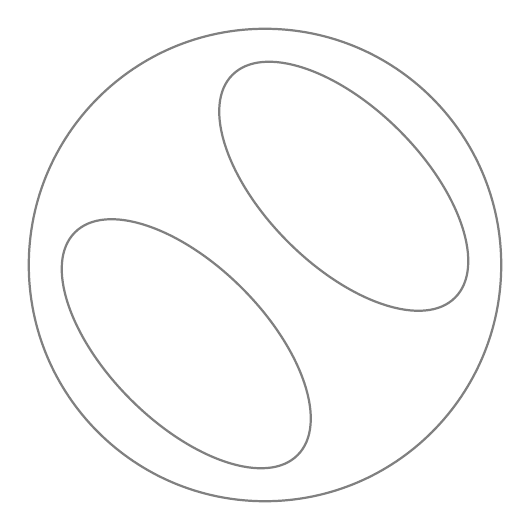
\begin{tikzpicture}
  \Vertex[x=2,y=4]{1}
  \Vertex[x=4,y=2]{2}
  \Vertex[x=2,y=0]{3}
  \Vertex[x=0,y=2]{4}
  \Edge[label=3](1)(2)
  \Edge[label=1](1)(4)
  \Edge[label=2,labelstyle={pos=0.8}](1)(3) %TODO: Labels above
  \Edge[label=2](2)(3)
  \Edge[label=2,labelstyle={pos=0.2}](2)(4)
  \Edge[label=4](3)(4)
  \draw[gray,thick,rotate around={-45:(3, 3)}] (3, 3) ellipse (2 and 1);
  \draw[gray,thick,rotate around={-45:(1, 1)}] (1, 1) ellipse (2 and 1);
  \draw[gray,thick] (2, 2) circle (3);
\end{tikzpicture}
  
\caption{Ejemplo de un archipiélago con todos los candidatos circulados.}
\label{fig:ej2-ex}
\end{figure}

\subsection{Algoritmo}
\label{sec:ej2-algorithm}
\paragraph{} Para encontrar todas las combinaciones candidatas aplicamos el algoritmo de árbol generador mínimo de \textbf{Kruskal}, que va armando un bosque construido por las aristas de mayor peso, y proponemos que en cada iteración que se agrega una arista la componente conexa que se expanda es una posible candidata. En la sección \ref{sec:ej2-proof} demostramos que este planteo es correcto. \\
Para decidir si cada componente es candidata y poder llevar la suma de sus tamaños, implementamos un \textbf{Disjoint Set} que para cada componente conexa del bosque lleva registro de su tamaño y de las aristas máxima y mínima hacia toda otra componente, donde la mínima hacia sigo misma es la mínima interna. Esto nos permite revisar si una componente es candidata revisando si la mínima interna es más grande que todas las máximas hacia las otras componentes en \(\bigO{n\alpha^{-1}(n)}\), ya que la cantidad de componentes es \(\bigO{n}\). \\
Como sólo revisamos si una componente es candidata cuando unimos dos componentes en Kruskal, y esto sucede \(\bigO{n}\) veces entonces esto suma \(\bigO{n^{2}\alpha^{-1}(n)}\) a la complejidad de Kruskal, dejando la complejidad del algoritmo en \(\bigO{Kruskal + n^{2}\alpha^{-1}(n)} = \bigO{mlog(n) + m\alpha^{-1}(n) +n^{2}\alpha^{-1}(n)} \overset{m \leq n^{2}}{=} \bigO{mlog(n) + n^{2}\alpha^{-1}(n)}\) que es igual a la complejidad de Kruskal.

\begin{figure}[H]
\centering

\begin{tikzpicture}
  \Vertex[x=0,y=8,L=4]{04}
  \Vertex[x=0,y=6,L=3]{03}
  \Vertex[x=-1,y=8,empty]{01}
  \Edge[label=4](04)(03)
  \Edge[label=1,style={color=red}](04)(01)

  \Vertex[x=2,y=8,L=2]{12}
  \Vertex[x=2,y=6,L=1]{11}
  \Vertex[x=1,y=8,empty]{13}
  \Edge[label=3](12)(11)
  \Edge[label=2,style={color=red}](12)(13)

  \Vertex[x=4,y=8,L=4]{24}
  \Vertex[x=4,y=6,L=3]{23}
  \Vertex[x=4,y=4,L=2]{22}
  \Vertex[x=4,y=2,L=1]{21}
  \Edge[](24)(23)
  \Edge[](22)(21)
  \Edge[label=2](23)(22)
\end{tikzpicture}
  
\caption{Las componentes que encuentra nuestro algoritmo sobre el grafo de la figura \ref{fig:ej2-ex} en orden. Con la arista interna mínima y la arista externa máxima resaltadas}
\label{fig:ej2-res}
\end{figure}

\subsubsection{Correctitud del algoritmo}
\label{sec:ej2-proof}
\paragraph{} Queremos contar los tamaños de todos los subconjuntos candidatos a \textit{Tour Belt} que tiene cierto Archipiélago conocido, representado con \(G = (V, E)\). Sabemos que para ser subconjunto \(B = (V', E')\) candidato (con $V' \subset V$ y $E' \subset E$), $|B|$ debe ser mayor o igual a 2, y los pesos de las aristas internas de $B$ deben ser mayores a los pesos de las aristas del borde de $B$. \\
En el modelo planteado, cada \textit{Tour} parcial puede verse como un bosque dentro de $G$. Entonces, si queremos encontrar todos los \textit{Tours} posibles de $G$, requerimos ir encontrando todos los bosques $B$ posibles que cumplan las condiciones mencionadas. Esto es exactamente lo que va haciendo el algoritmo de \textbf{Kruskal}. A partir del ordenamiento de las aristas por su peso, en forma descendente, se ir\'an conformando todos los bosques posibles que puedan ser \textit{Tours}. Veamos cómo es que se realiza esta parte. \\
Supongamos que estamos en la \textbf{iteración k} del algoritmo. Tomamos de $V$ la próxima arista, \(vk =(s,t)\), con \textit{s, t} vértices de $V$. Esta arista es aquella de mayor peso que todavía no fue considerada como efecto de sinergia, determinante para conformar un nuevo \textit{Tour Belt}. Será considerada, únicamente, si incluirla hace que exista una componente conexa menos en $G$. 
% Es decir, si al considerarla para conformar un nuevo Tour a partir de las dos islas que está uniendo, efectivamente la cantidad de componentes conexas de G, decrementa en una unidad, genera que haya un bosque menos en G. 
Esto podemos afirmarlo por el \textbf{invariante de Kruskal}. Tenemos dos escenarios posibles:
\begin{itemize}
  \item[\textbf{1)}] Si $s$ y $t$ no pertenecen todavía a ningún $B$ candidato a $Tour$, $vk$ será aquella sinergia que los convierta en candidatos válidos, ya que por la hipótesis del ordenamiento de las aristas, sabemos que no existe arista, de mayor peso que $vk$, que pueda llegar a estar en el borde de este nuevo $Tour$. Por lo tanto, $s$ y $t$ conforman un nuevo $B$ en $G$, y su tamaño será contabilizado. 
  \item[\textbf{2)}] Si $s$ o $t$, o $ambos$, ya pertenecen a algún $B \subset G$ previamente tenido en cuenta, $vk$ será nuevamente la mayor sinergia disponible, entre las demás sinergias candidatas. Por lo tanto, al incluirla tenemos la garantía de que la cantidad de bosques en $G$ va a disminuir (por el \textbf{invariante de Kruskal}), y que cualquier arista \textbf{no} perteneciente al nuevo $B$ %(producto de unir los dos Tours ya existentes que incluían a s y a t)
    costar\'a menos que las propias. Entonces, sus aristas del interior tendr\'an un costo mayor al de las aristas del borde. \\
  Con esto queda justificado que \textbf{Kruskal} nos ayuda a resolver el problema de \textit{Tour Belt}.
\end{itemize}

\end{document}
